% Chapter 3: Methodology and Results 
\chapter{Methodology and Experiments}
\label{ch:methodology}

This chapter details the methodological framework of our study. We first describe the creation of a synthetic dataset designed to test causal inference methods in a controlled environment. We then provide a comprehensive overview of the causal discovery algorithms employed. A central focus of this chapter is the detailed examination of the DIVOT (Distributional Inference of Variable Order with Transport) method, an approach that leverages optimal transport theory. Finally, we present the experimental results from applying these methods to our synthetic data, which serves to validate our framework before its application to real-world financial data in the subsequent chapter.

% Optimal transport is the unifying mathematical tool that threads through both estimation and discovery stages, and each method below applies it in a distinct way.

\section{Synthetic Data Generation}
To test our methods, we first need to create a synthetic dataset. This dataset is like a small, controlled world where we know the true answers. This helps us check if our methods work correctly. The dataset represents $N=100$ stocks over $T=48$ months. Each stock has four factors: Value, Size, Quality, and Volatility.

\begin{itemize}
    \item \textbf{Value}: Measures how cheap a stock is relative to fundamentals (e.g., book-to-market ratio). This factor has no real causal effect on returns. We include it as a test, like a placebo.
    \item \textbf{Size}: Represents market capitalization, where smaller companies historically show higher returns. This factor has a small positive effect (+0.5\% per standard deviation).
    \item \textbf{Quality}: Captures profitable companies with strong fundamentals (high earnings, low debt). This factor has a meaningful positive effect (+1\% per standard deviation). This is a known idea in finance.
    \item \textbf{Volatility}: Measures price variation and risk. This factor has a small negative effect (-0.5\% per standard deviation). Stocks with lower volatility often have higher risk-adjusted returns.
\end{itemize}
We set the true effects as follows. A one standard deviation increase in quality raises monthly returns by about 1\%. For size, the effect is 0.5\%. For volatility, the effect is negative 0.5\%. Value has a 0\% effect because it is a placebo. Importantly, we use the same beta coefficients for all stocks - every stock experiences the same +1\% return boost per standard deviation of quality exposure, though each stock has different factor exposures. Each stock also has a baseline return of 1\% per month and some random noise.

We created the factor data from a multivariate normal distribution with a carefully designed correlation structure. This lets us set realistic correlations between the factors that mirror patterns observed in empirical financial data. The correlation matrix we use is:

\begin{equation}
\mathbf{R} = \begin{pmatrix}
1.0 & 0.1 & -0.3 & 0.0 \\
0.1 & 1.0 & 0.2 & 0.4 \\
-0.3 & 0.2 & 1.0 & 0.1 \\
0.0 & 0.4 & 0.1 & 1.0
\end{pmatrix}
\end{equation}

where rows and columns represent Value, Size, Quality, and Volatility respectively. Key correlations include:
\begin{itemize}
    \item Quality is negatively correlated with Value (-0.3), reflecting that high-quality firms often trade at premium valuations
    \item Size is positively correlated with Volatility (0.4), as smaller stocks tend to be more volatile
    \item Quality has a modest positive correlation with Size (0.2), as larger companies often have stronger fundamentals
\end{itemize}

These patterns are similar to what we see in real financial research. All factors are standardized to have zero mean and unit variance.

We also added a treatment variable. This simulates an event that changes some of the stocks. At month 25, a "treatment" affects half of the stocks. This could be a new regulation or a market change.

The treatment was not random. We assigned treatment to stocks with higher quality scores. This creates a problem called confounding. It means the treated stocks are already different from the control stocks before the treatment. This makes it harder to find the true causal effect. Our methods must be good enough to solve this problem. A simple comparison of the treated and control groups would give a wrong answer because of this quality difference.

The treatment itself is a binary variable. It is 0 before month 25. After month 25, it is 1 for the treated stocks. The treatment adds a 5\% boost to the monthly returns of treated stocks. This is the true causal effect we want to find with our methods. The effect is large so it is easier to see the results in our analysis.

Quality is a confounder. It affects both treatment assignment and returns. This means treated stocks already have higher returns before the treatment because they have higher quality. This setup helps us test how well each causal method handles confounding. Figure~\ref{fig:confounder} shows this confounding problem.

\begin{figure}[ht]
\centering
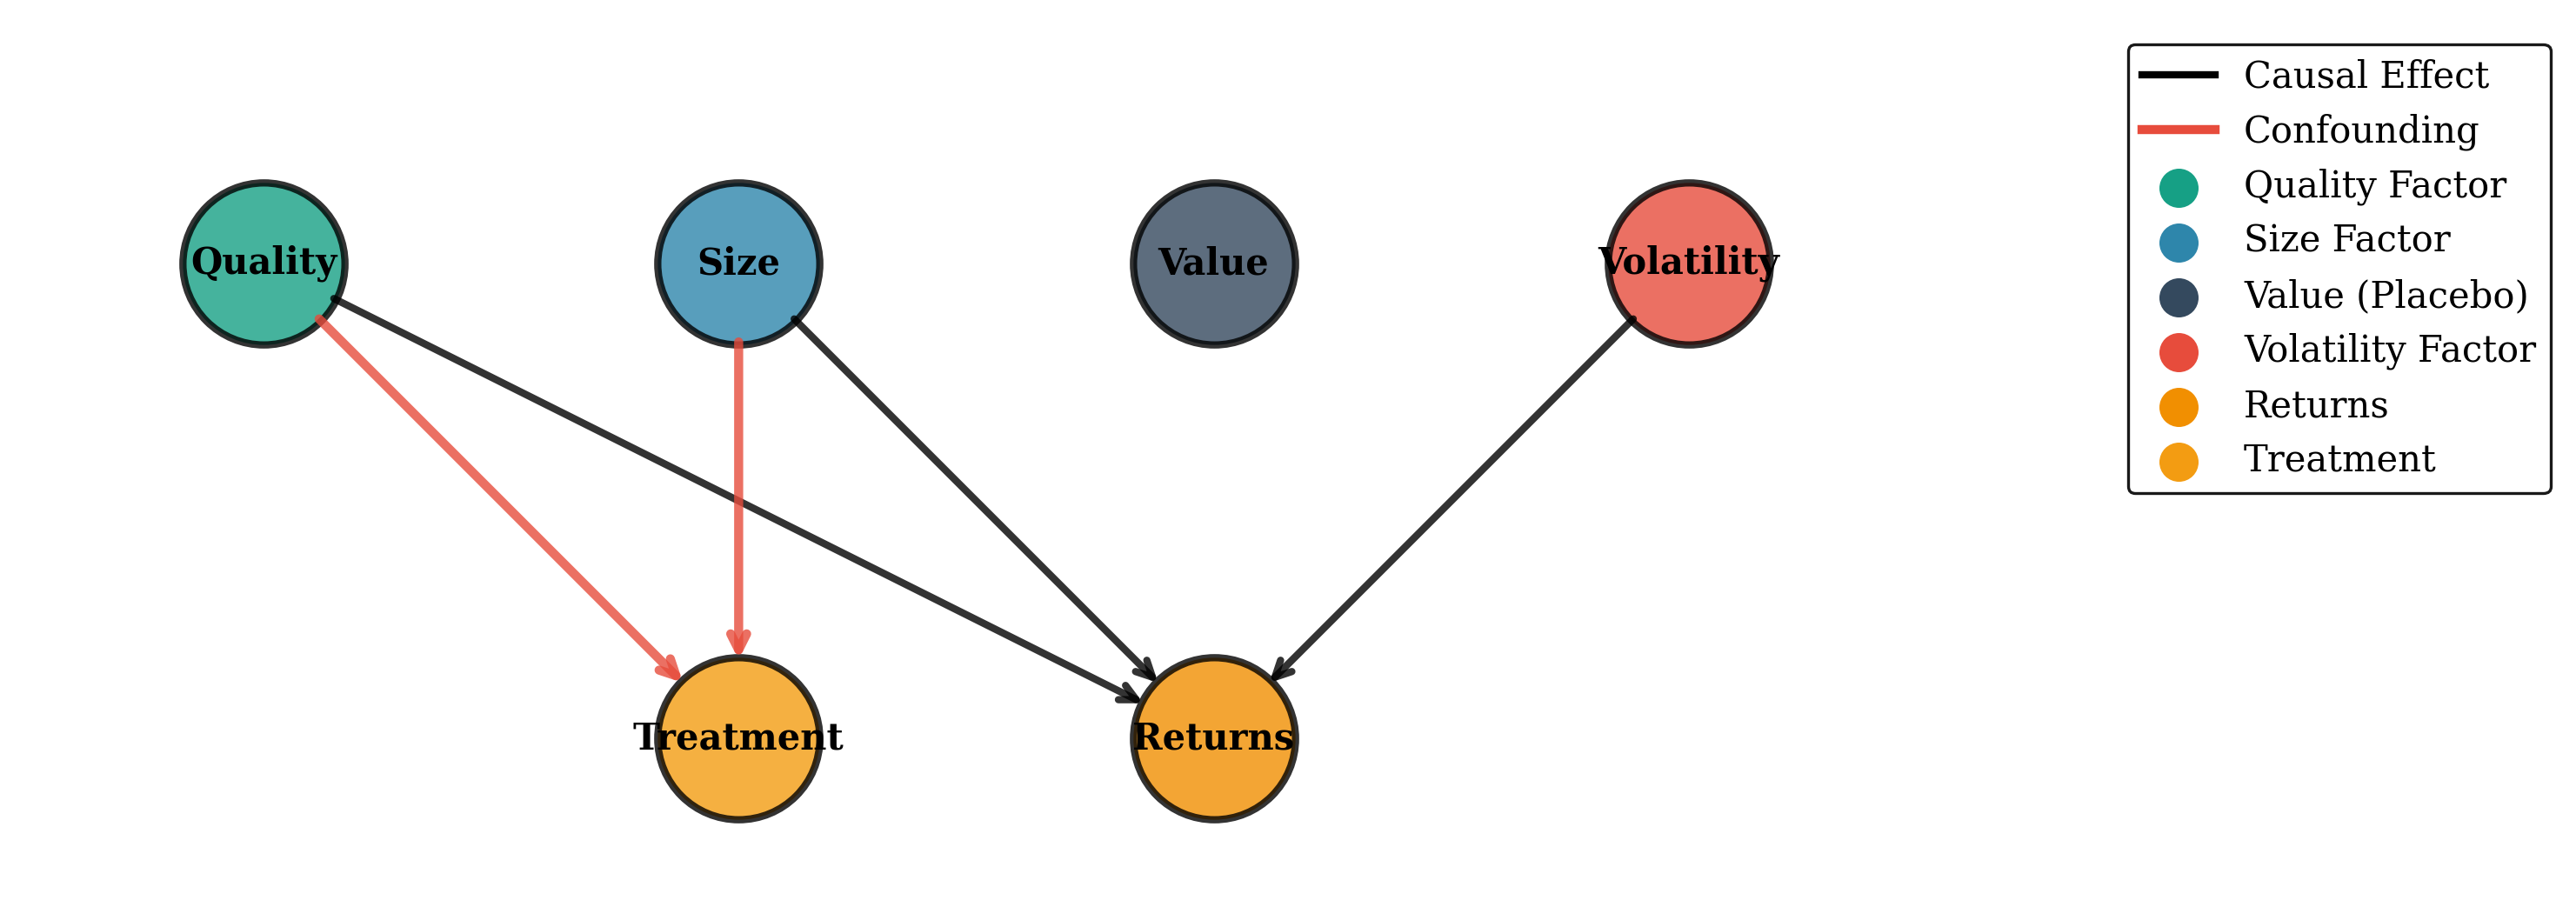
\includegraphics[width=0.85\textwidth]{Graphs/Synthetic/confounder_graph.png}
\caption{The confounding mechanism designed into the synthetic data. Quality is a common cause of both treatment assignment and returns, making it a confounder.}
\label{fig:confounder}
\end{figure}

Table~\ref{tab:sim_params} lists the key parameters for our simulation. We also created another dataset with no treatment effect at all. This is for a placebo test to make sure our methods do not find effects that are not there.

\begin{table}[ht]
\centering
\caption{Key Simulation Parameters}
\label{tab:sim_params}
\begin{tabular}{l l}
\hline
Baseline return ($\alpha$) & 0.01 (1\% per month) \\
Idiosyncratic noise std & 0.02 (2\%) \\
Quality factor effect ($\beta_{quality}$) & +0.01 per 1 s.d. (same for all stocks) \\
Size factor effect ($\beta_{size}$) & +0.005 per 1 s.d. (same for all stocks) \\
Volatility factor effect ($\beta_{volatility}$) & $-0.005$ per 1 s.d. (same for all stocks) \\
Value factor effect ($\beta_{value}$) & 0.0 (no effect; placebo factor) \\
Treatment effect & +0.05 (true +5\% return for treated stocks post-treatment) \\
Treatment group selection & Top 50 stocks by quality propensity (confounded) \\
\hline
\end{tabular}
\end{table}

\subsection*{Simulation Model and Data Generation}

Our synthetic data has a correlation structure that we designed on purpose. It reflects realistic factor relationships but with controlled causal effects. This section first describes the underlying model used to simulate returns and then discusses the data generation process.

\textbf{Return Generation Model}: The monthly return for each stock $i$ at time $t$, denoted $R_{i,t}$, is generated by a linear factor model. The goal of this model is to create a realistic, yet controlled, environment where we know the true causal relationships. This allows us to test our causal discovery algorithms against a known ground truth. The model includes four factors, a baseline return, a treatment effect, and idiosyncratic noise. The formula is:

\[
R_{i,t} = \alpha + \sum_{f} \beta_f \cdot F_{f,i} + \tau \cdot D_{i,t} + \epsilon_{i,t}
\]

where each component has a specific role in simulating stock returns:
\begin{itemize}
    \itemsep0em 
    \item \textbf{$R_{i,t}$ (Stock Return)}: The final output variable we are trying to understand and predict.
    \item \textbf{$\alpha$ (Baseline Return)}: This represents the average return of the market that is not explained by any of the factors. It's a constant drift term, ensuring that stocks have a positive expected return on average, reflecting the general upward trend of the market over time.
    \item \textbf{$\sum_{f} \beta_f \cdot F_{f,i}$ (Factor Effects)}: This is the core of the causal structure. For each stock $i$, we sum the effects of all its factor exposures. $F_{f,i}$ is the stock's factor exposure (e.g., its quality or size score), which varies by stock but is constant over time. The $\beta_f$ is the universal causal impact of that factor on returns - the same for all stocks. For example, all stocks get a +1\% return boost per standard deviation of quality exposure, but each stock has a different quality score. By setting these universal $\beta$ values, we embed the ground truth that our algorithms are designed to discover.
    \item \textbf{$\tau \cdot D_{i,t}$ (Treatment Effect)}: This term introduces a known causal shock into the system. It simulates a specific event (like a new policy or technology) that affects a subset of stocks (the "treated" group) after a certain point in time. It allows us to test methods that estimate the magnitude of a known intervention. In our model, this is a clear, unambiguous causal effect.
    \item \textbf{$\epsilon_{i,t}$ (Idiosyncratic Noise)}: This term represents the random, unpredictable component of a stock's return. It captures all the information that is not explained by the factors or the treatment, such as company-specific news or random market fluctuations. This noise makes the causal discovery task more challenging and realistic, as real-world financial data is inherently noisy.
\end{itemize}

By combining these elements, the model generates a synthetic dataset that mirrors the key characteristics of real financial markets, including underlying trends, factor-driven returns, specific events, and randomness, while still providing a controlled environment where we know the true causal links. This is essential for validating our causal discovery framework.

\textbf{Data Generation Process}: The simulation follows these steps:
\begin{enumerate}
    \itemsep0em 
    \item \textbf{Factor Generation}: We generate the time-invariant factor exposures for all $N=100$ stocks. The four factor values for each stock are drawn from a multivariate normal distribution with a mean of zero and the specified correlation matrix.
    \item \textbf{Treatment Assignment}: Treatment is assigned based on the Quality factor to introduce confounding. A stock's probability of being treated (its propensity) increases with its quality score. The 50 stocks with the highest propensity are assigned to the treated group.
    \item \textbf{Return Calculation}: For each of the $T=48$ months, we calculate each stock's return using the linear model described above. The idiosyncratic noise $\epsilon_{i,t}$ is drawn independently for each stock in each month.
\end{enumerate}

This process creates a panel dataset where the causal links are known, allowing us to test our methods against a ground truth. The confounding between Quality and treatment assignment provides a realistic challenge for the causal inference algorithms.

\section{Causal Discovery Algorithms}
\label{sec:methodologies}

% Roadmap sentence for clarity
This section details the causal discovery algorithms used in our study. Our analysis compares several established methods against DIVOT, an approach based on optimal transport that is a core focus of this thesis.

\subsection{Causal Discovery Algorithms}

These algorithms are used to discover the direction of unknown causal relationships from observational data. Our analysis compares several established methods against DIVOT, an approach based on optimal transport that is a core focus of this thesis.

\subsubsection{PC Algorithm}
To provide a baseline from classical causal discovery, we use the Peter-Clark (PC) algorithm, a standard "constraint-based" method for learning causal graphs from data \cite{Spirtes00}. The algorithm works in two main phases: first finding the graph's structure, and then determining the direction of the connections.

\textbf{Phase 1: Skeleton Discovery}. The algorithm starts with a graph where every variable is connected. It then uses statistical tests to remove connections. For any two variables, $X$ and $Y$, the algorithm checks if they are independent given another set of variables, $S$. If they are independent, the connection is removed:
\[
\text{If } (X \perp Y \mid S), \text{ then remove the edge between } X \text{ and } Y.
\]
This process is repeated many times, using different sets of variables for $S$. In our implementation, we use Fisher's Z-transform for these tests, with a significance level of $\alpha = \GlobalAlphaLevel$. This phase stops when no more connections can be removed. The result is the basic structure, or "skeleton," of the graph.

\textbf{Phase 2: Edge Orientation}. After finding the skeleton, the algorithm determines the direction of the remaining connections. It does this by looking for specific patterns called "v-structures" (or colliders). A v-structure looks like $X \rightarrow Z \leftarrow Y$. Finding these v-structures helps the algorithm to orient the other edges in the graph. The final result is a directed graph that shows the causal relationships.

\subsubsection{Additive Noise Model (ANM)}
To get a different view, we used the Additive Noise Model (ANM), following the work of Hoyer et al. (2009)\cite{Hoyer09}. This method tests for causal relationships between pairs of variables. It is based on the principle that if $X$ causes $Y$, the relationship can be written as:
$$Y = f(X) + \epsilon$$
where $f$ is some function, and the noise term $\epsilon$ is independent of the cause $X$. The key idea is that this independence of the noise only holds in the true causal direction.

The causal direction is inferred to be the one where the independence condition holds more strongly. If both directions show similar levels of independence (or dependence), the result is considered inconclusive. This asymmetry provides the basis for determining causality.

To ensure robustness, our implementation uses two key enhancements:
\begin{enumerate}
    \item \textbf{Gaussian Process Regression}: Instead of assuming a simple linear function, we use a more flexible Gaussian Process to model the function $f(X)$.
    \item \textbf{Distance Correlation for Independence}: We test for independence using distance correlation, a powerful statistical tool that can detect both linear and non-linear dependencies between variables.
\end{enumerate}
By using these more advanced techniques, our ANM implementation is better at finding the correct causal direction, even in complex situations where simple linear models would fail.

\subsubsection{ANM Decision Criteria}

The ANM method compares the independence of residuals in both causal directions. To decide the direction, we calculate an independence score (specifically, the distance correlation) for each case:
\begin{itemize}
    \item For $X \rightarrow Y$: Independence score between $X$ and residuals from $Y \sim f(X) + \epsilon$
    \item For $Y \rightarrow X$: Independence score between $Y$ and residuals from $X \sim g(Y) + \eta$
\end{itemize}

A lower score indicates stronger independence. The algorithm decides the causal direction based on which score is significantly lower, using a small threshold to avoid making decisions based on statistical noise:
\begin{align}
\text{Direction} = \begin{cases}  
X \rightarrow Y & \text{if } \text{score}(X \rightarrow Y) < \text{score}(Y \rightarrow X) - \text{threshold} \\
Y \rightarrow X & \text{if } \text{score}(Y \rightarrow X) < \text{score}(X \rightarrow Y) - \text{threshold} \\
\text{Inconclusive} & \text{otherwise}
\end{cases}
\end{align}

\subsubsection{DIVOT: Causal Discovery with Optimal Transport}
A core contribution of this thesis is the application and analysis of the DIVOT (Distributional Inference of Variable Order with Transport) method. This approach uses optimal transport theory to find causal direction, following the ideas from Tu et al. (2022)\cite{Tu22}. The main idea is that the true causal direction shows a simpler or more "efficient" pattern when we look at it through the lens of optimal transport. This builds on other research that uses optimal transport for causal inference\cite{Charpentier23,Torous24}.

Our DIVOT implementation is based on the framework from Tu et al. (2022) and uses three different signals to find the causal direction\cite{Tu22}:
\begin{enumerate}
    \item \textbf{Transport Cost Asymmetry}: We calculate the Wasserstein-2 distance between the factor and return distributions. The formula for the Wasserstein-2 distance between two distributions $\mu$ and $\nu$ is:
    $$W_2(\mu, \nu) = \left( \inf_{\gamma \in \Pi(\mu,\nu)} \int_{\mathbb{R} \times \mathbb{R}} \|x - y\|^2 d\gamma(x,y) \right)^{1/2}$$
    Here, $\Pi(\mu,\nu)$ is the set of all joint distributions whose marginals are $\mu$ and $\nu$. The formula finds the "cheapest" way to move the probability mass of $\mu$ to match the distribution of $\nu$.

    \item \textbf{Residual Independence Asymmetry}: We use the same robust independence test that we used in our ANM analysis (distance correlation). The direction with more independent residuals is more likely to be the true causal direction.

    \item \textbf{Transport Map Smoothness Asymmetry}: We look at the entropy of the optimal transport plan, $\gamma$. A smoother, more structured plan has lower entropy. A lower entropy suggests a more natural, and therefore more likely, causal relationship. We can use entropic regularization, as suggested by Cuturi (2013), to help find these smoother plans by solving for:
    $$W_{\lambda}(\mu, \nu) = \inf_{\gamma \in \Pi(\mu,\nu)} \left[\int c(x,y) d\gamma(x,y) + \lambda H(\gamma)\right]$$
    where $c(x,y)$ is the cost, $H(\gamma)$ is the entropy of the transport plan, and $\lambda$ is a regularization parameter\cite{Cuturi13}.
\end{enumerate}

The final decision is based on a weighted score from these three parts, as proposed by Tu et al. (2022).
$$S_{DIVOT} = 0.4 \cdot \Delta_{transport} + 0.4 \cdot \Delta_{independence} + 0.2 \cdot \Delta_{smoothness}$$
This multi-part approach makes our DIVOT method more robust than simpler methods. Unlike PC and ANM, DIVOT's score is explicitly distributional and grounded in optimal transport, offering a complementary perspective on causality in factor investing.

\subsubsection{DIVOT Confidence Thresholds}
Our DIVOT implementation uses a systematic scoring rule that combines three types of evidence:

\begin{enumerate}
    \item \textbf{Transport Cost Evidence} (40\% weight): Lower Wasserstein distance shows more efficient mapping
    \item \textbf{Residual Independence Evidence} (40\% weight): Lower distance correlation between predictor and residuals shows better causal fit  
    \item \textbf{Smoothness Evidence} (20\% weight): Lower entropy in transport plans shows more structured mapping
\end{enumerate}

The final direction score is computed as:
$$S_{DIVOT} = 0.4 \cdot \Delta_{transport} + 0.4 \cdot \Delta_{residual} + 0.2 \cdot \Delta_{smoothness}$$
where $\Delta$ represents the difference between Y$\rightarrow$X and X$\rightarrow$Y metrics. A positive score indicates X$\rightarrow$Y causality, while a negative score indicates Y$\rightarrow$X.

\textbf{Decision Rule}: We classify directions based on the magnitude of the score:
\begin{itemize}
    \item $|S_{DIVOT}| > 0.002$: The evidence is strong enough to assign a causal direction with \textbf{Moderate} confidence.
    \item $|S_{DIVOT}| \leq 0.002$: The evidence is weak, and the result is deemed \textbf{Inconclusive} (Low confidence).
\end{itemize}

This scoring system proved effective in our analysis. The method's strength derives from its integration of multiple sources of evidence, leveraging optimal transport theory to detect the natural flow of causal influence between variables.

\section{Experimental Results on Synthetic Data}
\label{sec:synthetic_results}

This section presents the results from applying our suite of causal methods to the synthetic dataset. The known ground truth of the data allows us to rigorously evaluate the performance of each method.

\subsection{Causal Discovery Results}
This section uses several different approaches to find out which factors are real drivers of returns.

\subsubsection{PC Algorithm Results}
The PC algorithm achieved \SyntheticPCAccuracy{} accuracy in our synthetic test. It correctly identified that the "Value" factor has no causal link to returns, and it also correctly found the causal links for the Size and Volatility factors. However, it failed to identify the true causal relationship for the Quality factor, likely due to the strong confounding effect we designed into the data.

\begin{table}[ht]
\centering
\caption{PC Algorithm Causal Discovery Results}
\label{tab:pc_results}
\begin{tabular}{lccc}
\toprule
\textbf{Factor} & \textbf{PC Result} & \textbf{True Direction} & \textbf{Correct} \\
\midrule
Value & Not identified as cause & None (placebo) & \checkmark \\
Size & Size $\rightarrow$ Returns & Size $\rightarrow$ Returns & \checkmark \\
Quality & Not identified as cause & Quality $\rightarrow$ Returns & \ding{55} \\
Volatility & Volatility $\rightarrow$ Returns & Volatility $\rightarrow$ Returns & \checkmark \\
\midrule
\textbf{Accuracy} & \multicolumn{3}{c}{\textbf{\SyntheticPCAccuracy}} \\
\bottomrule
\end{tabular}
\end{table}

\textbf{PC Algorithm Performance}:
\begin{itemize}
    \item \textbf{Correct Identifications}: The PC algorithm successfully identified three of the four causal relationships. It correctly found the causal direction for the Size and Volatility factors, and also correctly identified that the Value (placebo) factor has no effect.
    \item \textbf{Missed Relationship}: It only failed to find the true causal link for the Quality factor. This is a very strong performance for the algorithm on this dataset.
\end{itemize}

\subsubsection{ANM Results}
Table~\ref{tab:anm_results_enhanced} presents the ANM results. The method achieved \SyntheticANMAccuracy{} accuracy. It correctly identified the direction for the Size factor, but it gave incorrect or inconclusive results for the other three factors. This poor performance suggests that ANM, even with the Gaussian Process Regression implementation, struggled to find the causal relationships in our synthetic financial data.

\begin{table}[ht]
\centering
\caption{ANM Causal Discovery Results vs. Ground Truth*}
\label{tab:anm_results_enhanced}
\begin{tabular}{lccc}
\toprule
\textbf{Factor} & \textbf{ANM Prediction} & \textbf{Ground Truth} & \textbf{Correctness} \\
\midrule
Value & Value $\rightarrow$ Returns & None (placebo) & \ding{55} \\
Size & Size $\rightarrow$ Returns & Size $\rightarrow$ Returns & \checkmark \\
Quality & Inconclusive & Quality $\rightarrow$ Returns & \ding{55} \\
Volatility & Returns $\rightarrow$ Volatility & Volatility $\rightarrow$ Returns & \ding{55} \\
\midrule
\textbf{Accuracy} & \multicolumn{3}{c}{\textbf{\SyntheticANMAccuracy}} \\
\bottomrule
\end{tabular}
\end{table}

\subsubsection{DIVOT Results}
The DIVOT algorithm, which uses optimal transport, had mixed results on the synthetic data, achieving \SyntheticDivotAccuracy{} accuracy. While it successfully identified the causal direction for the Size and Quality factors, it made errors on the Value and Volatility factors. The error on the Value (placebo) factor is a notable failure, as it suggests the method may be prone to finding causal links where none exist.

\begin{table}[ht]
\centering
\caption{DIVOT Causal Discovery Results vs. Ground Truth}
\label{tab:divot_results}
\begin{tabular}{lccc}
\toprule
\textbf{Factor} & \textbf{DIVOT Prediction} & \textbf{Ground Truth} & \textbf{Correctness} \\
\midrule
Value & Value $\rightarrow$ Returns & None (placebo) & \ding{55} \\
Size & Size $\rightarrow$ Returns & Size $\rightarrow$ Returns & \checkmark \\
Quality & Quality $\rightarrow$ Returns & Quality $\rightarrow$ Returns & \checkmark \\
Volatility & Returns $\rightarrow$ Volatility & Volatility $\rightarrow$ Returns & \ding{55} \\
\midrule
\textbf{Accuracy} & \multicolumn{3}{c}{\textbf{\SyntheticDivotAccuracy}} \\
\bottomrule
\end{tabular}
\end{table}

\subsection{Summary of Method Performance}

\begin{table}[ht]
\centering
\caption{Overall Comparison of Causal Discovery Methods on Synthetic Data}
\label{tab:causal_methods_comparison}
\begin{tabular}{lccc}
\toprule
\textbf{Method} & \textbf{Accuracy} & \textbf{Identified Placebo} & \textbf{Notes} \\
\midrule
PC Algorithm & \SyntheticPCAccuracy & Yes & Strongest performer, but missed one link \\
DIVOT & \SyntheticDivotAccuracy & No & Found two links, but failed on placebo \\
ANM & \SyntheticANMAccuracy & No & Weakest performer, struggled with confounding \\
\bottomrule
\end{tabular}
\end{table}

The results show that the PC algorithm was the most reliable on our synthetic data. DIVOT showed promise but needs to be used with caution, as it incorrectly identified the placebo factor as causal. ANM's performance suggests it may not be well-suited for this type of financial data. These findings provide a crucial baseline before we apply the methods to more complex real-world data in the next chapter.